\documentclass[12pts, letterpaper]{article}

\usepackage[utf8]{inputenc}
\usepackage{amsmath}
\usepackage{amssymb}
\usepackage{amsthm}
\usepackage{amsfonts}
\usepackage{physics}
\usepackage{enumerate}
\usepackage{graphicx}
\graphicspath{ {images/} }
\usepackage[margin=1in]{geometry}
\usepackage{fancyhdr}
\usepackage{sectsty}
\subsubsectionfont{\centering}

\lhead{\sffamily{Quantum Information and Quantum Computation}}
\rhead{\sffamily{Vibhav Aggarwal}}
\cfoot{\sffamily{\thepage}}
\numberwithin{equation}{section}
\theoremstyle{definition}
\newtheorem{theorem}{Theorem}
\newtheorem{postulate}{Postulate}
\newtheorem{lemma}[theorem]{Lemma}
\newtheorem{corollary}[theorem]{Corollary}
\newtheorem{definition}{Definition}
\numberwithin{definition}{section}
\numberwithin{theorem}{section}
\newtheorem*{thesis}{Thesis}
\newtheorem{exercise}{Exercise}
\newtheorem*{example}{Example}

\theoremstyle{remark}
\numberwithin{exercise}{section}
\newtheorem*{solution}{Solution}
\pagestyle{fancy}

\setcounter{section}{-1}

\setlength\parindent{0pt}
\title{Quantum Information and Quantum Computation}
\author{Vibhav Aggarwal\thanks{Mentored by Neeraj Sohani}}
\date{June 2020}

\begin{document}

\maketitle

\tableofcontents
\newpage
\section{Introduction}

Quantum computation and quantum information is the study of the information processing tasks that can be accomplished using quantum mechanical systems. It is relatively a newer field of research and much work is going on to actually make a functional quantum computer. Big tech companies like Google, Microsoft, Hitachi, Mitsubishi, Nokia, etc. are investing huge amounts of money in research and development of quantum computers.
\vspace{1em}

But why? What is so special about this field that so many people are interested in it? Turns out, quantum computers offer an essential speed advantage over classical computers. This speed advantage is so significant that many researchers believe that no conceivable amount of progress in classical computation would be able to overcome the gap between the power of a classical computer and the power of a quantum computer!
\vspace{1em}

For example, the RSA cryptosystem used for transferring data in secure manner is just based on the fact that it is very difficult for a classical computer to factorize large numbers (order of 2048 bits) quickly. Till date there is simply no known algorithm to that efficiently on a classical computer. However, there is an algorithm known as Shor’s algorithm which can just do that really quickly on a quantum computer.
\vspace{1em}

There are many other algorithms based upon quantum computers and one class of such algorithms is the \textit{quantum search algorithms}. The quantum search algorithm solves
the following problem: Given a search space of size $N$, and no prior knowledge about the
structure of the information in it, we want to find an element of that search space satisfying a known property. How long does it take to find an element satisfying that property?
Classically, this problem requires approximately $N$ operations, but the quantum search algorithm allows it to be solved using approximately $\sqrt{N}$ operations.
\vspace{1em}

Another important use is \textit{quantum simulation}. Simulation of quantum systems on classical machines is difficult and the space requirement grows exponentially with increasing number of components in the system. But in case of quantum computers, this growth is linear and therefore they can be used in quantum chemistry to simulate large molecules and study the inter-atomic interactions.

\newpage
\section{Quantum bits (qubits)}

The \textit{bit} is the fundamental concept of classical computation. It has only two possible states: $0$ and $1$. Any information can be represented by a combination of bits. Using $n$ bits, a total of $2^n$ different messages can be represented/conveyed.
\\\\
Quantum computation and quantum information are built upon an analogous concept, the \textit{quantum bit}, or \textit{qubit} for short. Qubits are mathematical objects with certain properties. While it is true that qubits, like bits, are realized as actual physical systems, we are going to treat them as abstract mathematical objects.
\\\\
A qubit has a state, just like a bit, represent by $\ket{\psi}$. Two possible states are $\ket{0}$ and $\ket{1}$. However it can also have a state which is a linear combination of these two. Thus:
\begin{center}
    $\ket{\psi}=\alpha\ket{0} + \beta\ket{1}$
\end{center}

The numbers $\alpha$ and $\beta$ are complex numbers. Put another way, the state of a qubit is a vector in a two-dimensional complex vector space. The special states $\ket{0}$ and $\ket{1}$ are known as computational basis states, and form an \textit{orthonormal} basis for this vector space.
\\\\
Since $\alpha$ and $\beta$ can take infinitely many different complex values, one might be tempted to think that infinite different messages can be conveyed using a single qubit! But there's a catch. When we make a measurement of a qubit, its state \textit{collapses} into either $\ket{0}$ with probability $|\alpha|^2$ or $\ket{0}$ with probability $|\beta|^2$. So every time we observe only one of the two possible states. Naturally, $|\alpha|^2 + |\beta|^2 = 1$. 
\\\\
Geometrically, we can interpret this as the condition that the qubit’s state be normalized to length $1$. Thus, in general a qubit’s state is a unit vector in a two-dimensional complex vector space.
\\\\
Since $\alpha$ and $\beta$ are complex numbers with the only constraint that $|\alpha|^2 + |\beta|^2 = 1$, we may represent the state of qubit as:
    $$\ket{\psi} = e^{i\gamma}\left(\cos{\frac{\theta}{2}}\ket{0} + e^{i\phi}\sin{\frac{\theta}{2}}\ket{1}\right)$$

In fact, we can ignore the factor $e^{i\gamma}$ because it has no observable effects. Thus we can effectively write:
    $$\ket{\psi} = \cos{\frac{\theta}{2}}\ket{0} + e^{i\phi}\sin{\frac{\theta}{2}}\ket{1}$$

The numbers $\theta$ and $\phi$ define a point on the unit three-dimensional sphere, as shown in the figure below. This sphere is often called the \textit{Bloch sphere}.
\begin{figure}[h]
    \centering
    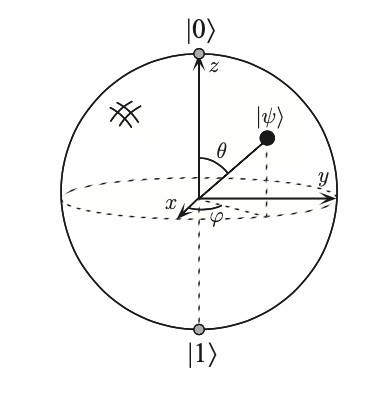
\includegraphics[width=0.35\textwidth]{bloch.png}
    \caption{Bloch sphere}
\end{figure}

\newpage
\section{Introduction to Quantum Mechanics}
To understand the concepts of quantum information and computing, a thorough understanding of quantum mechanics is required. Thus we must first get familiar with the mathematics involved and later we will see the postulates of quantum mechanics.

\subsection{Linear Algebra}
Linear algebra is the study of vector spaces and of linear operations on those vector spaces. A good understanding of quantum mechanics is based upon a solid grasp of elementary linear algebra.
\begin{definition}
    A \textit{spanning set} for a vector space is a set of vectors $\ket{v_1},\ldots,\ket{v_n}$ such that any vector $\ket{v}$ in the vector space can be written as a linear combination $\ket{v} = \sum_{i}{a_i\ket{v_i}}$ of vectors in that set. 
\end{definition}
\begin{definition}
    A \textit{linear operator} between vector spaces $V$ and $W$ is defined to be any function $A \colon\ V\ \rightarrow\ W$ which is linear in its inputs, $$A\left(\sum_{i}{a_i\ket{v_i}}\right)=\sum_{i}{a_iA\left(\ket{v_i}\right)}$$
\end{definition}
\\
The most convenient way to understand linear operators is in terms of their \textit{matrix representation}. Suppose $A \colon\ V\ \rightarrow\ W$ is a linear operator between vector spaces $V$ and $W$. Suppose $\ket{v_1},\ldots,\ket{v_m}$ is a basis for $V$ and $\ket{w_1},\ldots,\ket{w_n}$ is a basis for $W$ . Then for each $j$ in the range $1,\ldots,m$, there exist complex numbers $A_{1j}$ through $A_{nj}$ such that
    $$A\ket{v_j} = \sum_{i = 1}^{n}{A_{ij}\ket{w_i}}$$

The $n\times m$ matrix whose entries are the values $A_{ij}$ is said to form a matrix representation of the operator $A$.

Matrix representation is very helpful in the way that applying operator A to a vector $\ket{v}$ is equivalent to multiplying the matrix of $A$ by the column vector representation of $\ket{v}$.

\subsubsection*{The Pauli matrics}
Four extremely useful matrices are the Pauli matrices. They are defined as:
\begin{align*}
    \sigma_0\equiv\ I\equiv\begin{bmatrix}1&0\\0&1\\\end{bmatrix} && \sigma_1\equiv\sigma_x\equiv\ X\equiv\begin{bmatrix}0&1\\1&0\\\end{bmatrix}\\
    \sigma_2\equiv\sigma_y\equiv\ Y\equiv\begin{bmatrix}0&-i\\-i&0\\\end{bmatrix} && \sigma_3\equiv\sigma_z\equiv\ Z\equiv\begin{bmatrix}1&0\\0&-1\\\end{bmatrix}
\end{align*}

\subsubsection{Inner Products}
An \textit{inner product} is a function which takes as input two vectors $\ket{v}$ and $\ket{w}$ from a vector space and produces a complex number as output. For the time being, it will be convenient to write the inner product of $\ket{v}$ and $\ket{w}$ as $\left(\ket{v}, \ket{w}\right)$ although the standard quantum mechanical notation is $\braket{v}{w}$.
\\\\
A function $(\cdot, \cdot)$ from $V \cross V$ to $C$ is an inner product if it satisfies the requirements that:
\begin{enumerate}
    \item $(\cdot, \cdot)$ is linear in the second argument,
        $$\left(\ket{v}, \sum_{i}{\lambda_i\ket{w_i}}\right) = \sum_{i}{\lambda_i\left(\ket{v}, \ket{w_i}\right)}$$
    \item $\left(\ket{v}, \ket{w}\right) = \left(\ket{w}, \ket{v}\right)^\ast$
    \item $\left(\ket{v}, \ket{v}\right) \geq 0$ with equality if and only if $\ket{v} = 0$
\end{enumerate}

A vector space having an inner product is called an \textit{inner product space}.

For example, $\mathbb{C}^n$ has an inner product defined by
    $$((y_1,\ldots,y_n), (z_1,\ldots,\z_n)) = \sum_{i}{y_i^\ast z_i} = \begin{bmatrix}y_1^\ast & \dots & y_n^\ast\end{bmatrix} \begin{bmatrix}z_1 \\ \vdots \\ z_n\end{bmatrix}$$
\\\\
In the finite dimensional complex vector spaces that come up in quantum computation and quantum information, a \textit{Hilbert space} is \textit{exactly the same thing} as an inner product space. From now on we may use the two terms interchangeably.
\\\\
\begin{definition}
    Vectors $\ket{v}$ and $\ket{w}$ are \textit{orthogonal} if their inner product is zero.
\end{definition}
\begin{definition}
    The \textit{norm} of a vector is defined as,
        $$\norm{\ket{v}} = \sqrt{\braket{v}{v}}$$
\end{definition}
\begin{definition}
    A \textit{unit vector} is a vector $\ket{v}$ such that $\norm{\ket{v}} = 1$.
\end{definition}

\subsubsection{Eigenvectors and eigenvalues}
\begin{definition}
    An \textit{eigenvector} of a linear operator $A$ on a vector space is a non-zero vector $\ket{v}$ such that $A\ket{v} = v\ket{v}$, where $v$ is a complex number known as the \textit{eigenvalue} of $A$ corresponding to $\ket{v}$.
\end{definition}
\begin{definition}
    A \textit{diagonal representation} for an operator $A$ on a vector space $V$ is a representation $A = \sum_{i}{\lambda_i\ket{i}\bra{i}}$, where the vectors $\ket{i}$. form an orthonormal set of eigenvectors for $A$, with corresponding eigenvalues $\lambda_i$. Diagonal representations are sometimes also known as \textit{orthonormal decompositions}.
\end{definition}
\begin{definition}
    An operator is said to be \textit{diagonalizable} if it has a diagonal representation.
\end{definition}

\subsubsection{Adjoint and Hermitian operators}
\begin{definition}
    Suppose $A$ is any linear operator on a Hilbert space, $V$. There exists a unique operator $A^\dag$ on $V$ such that for all vectors $\ket{v}, \ket{w}\in V$, $(\ket{v}, A\ket{w}) = (A^\dag\ket{v}, \ket{w})$. The linear operator $A^\dag$ is known as the \textit{adjoint} or \textit{Hermitian conjugate} of the operator A.
\end{definition}
It can be proved that $A^\dag = (A^\ast)^T$
\begin{definition}
    An operator $A$ is said to be \textit{normal} if $AA^\dag=A^\dag A$.
\end{definition}
\begin{definition}
    An operator $A$ is said to be \textit{unitary} if $AA^\dag=\ I$.
\end{definition}
\begin{theorem}
    \textbf{(Spectral decomposition)} Any normal operator $M$ on a vector space $V$ is diagonal with respect to some orthonormal basis for $V$. Conversely, any diagonalizable operator is normal.
\end{theorem}
\begin{exercise}
    Show that a normal matrix is Hermitian if and only if it has real eigenvalues.
\end{exercise}
\begin{solution}
    $\left(\Longrightarrow\right)\tab$ Let $A\ket{v} = \lambda\ket{v}$. We have,
    \begin{equation*}
    \begin{split}
        (\ket{v}, A\ket{V}) & = (A^\dag\ket{v}, \ket{v}) \\
        (\ket{v}, \lambda\ket{v}) & = (\lambda\ket{v}, \ket{v}) \\
        \lambda(\ket{v}, \ket{v}) & = \lambda^*(\ket{v}, \ket{v}) \\
        \lambda & = \lambda^*
    \end{split}
    \end{equation*}
    
    $\left(\Longleftarrow\right)\tab$ By the spectral theorem, if $A$ is normal, then it is diagonalizable. Hence, $A=UDU^\dag$ for some unitary operator matrix $U$ and a diagonal matrix $D$ containing eigenvalues of $A$. Taking adjoint on both sides,
    \begin{equation*}
    \begin{split}
        A^\dag & = \left(UDU^\dag\right)^\dag \\
        & = UD^\ast U^\dag \\
        & = UDU^\dag \\
        & = A
    \end{split}
    \end{equation*}
\end{solution}

\begin{exercise}
    Show that all eigenvalues of a unitary matrix have modulus $1$, that is, can be written in the form $e^{i\theta}$ for some real $\theta$.
\end{exercise}
\begin{solution}
    \begin{equation*}
    \begin{split}
        U\ket{v} & = \lambda\ket{v} \\
        \implies \bra{v}U^\dag & = \bra{v}\lambda^\ast
    \end{split}
    \end{equation*}
    By multiplying the above equations, we get
    \begin{equation*}
    \begin{split}
        \bra{v}U^\dag U\ket{v} & = \bra{v}\lambda^\ast\lambda\ket{v} \\
        \braket{v}{v} & = \norm{\lambda}^2\braket{v}{v} \\
        \norm{\lambda}^2 & = 1 \\
        \norm{\lambda} & = 1
    \end{split}
    \end{equation*}
\end{solution}

\begin{definition}
    A positive operator $A$ is defined to be an operator such that for any vector $\ket{v}$, $(\ket{v}, A\ket{v})$ is a real, non-negative number.
\end{definition}

\begin{exercise}
    Show that a positive operator is necessarily Hermitian.
\end{exercise}
\begin{solution}
    Let
    \begin{align*}
        B = \frac{A+A^\dag}{2} && C = \frac{-iA+iA^\dag}{2}
    \end{align*}
    Then $B$ and $C$ are Hermitian and $A = B + iC$
    Hence
    $$\bra{v}A\ket{v} = \bra{v}B\ket{v} + i\bra{v}C\ket{v}$$
    Any Hermitian $X$ can be represent as $X = \sum_{i}{\lambda_i\ket{i}\bra{i}}$ where $\ket{i}$ are its eigenvectors and $\lambda_i$ are corresponding eigenvalues.
    For any vector $\ket{v}$, $\bra{v}X\ket{v} = \sum_{i}{\lambda_i\braket{v}{i}\braket{i}{v}}$ which is always real.
    Hence $\bra{v}C\ket{v} = 0$ for all vectors $\ket{v}$ and this combined with the fact that $C$ is Hermitian yields that $C$ is identically $0$. Therefore, $A$ must be Hermitian.
\end{solution}

\subsubsection{Tensor products}
The \textit{tensor product} is a way of putting vector spaces together to form larger vector spaces. This construction is crucial to understanding the quantum mechanics of multiparticle systems.
\\\\
In layman terms, tensor product of two vectors \textit{from different vector spaces} is simply the "concatenation" of these vectors (i.e. placing next to each other).
\\\\
Suppose $V$ and $W$ are vector spaces of dimension $m$ and $n$ respectively. For convenience we also suppose that $V$ and $W$ are Hilbert spaces. Then $V \otimes W$ (read '$V$ tensor $W$') is an $mn$ dimensional vector space. The elements of $V \otimes W$ are linear combinations of 'tensor products' $\ket{v}\otimes\ket{w}$ of elements $\ket{v}$ of $V$ and $\ket{w}$ of $W$. In particular, if $\ket{i}$ and $\ket{j}$ are orthonormal bases for the spaces $V$ and $W$ then $\ket{i}\otimes\ket{j}$ is a basis for $V \otimes W$.
\\\\
Tensor product can be defined for operators too. Let $A$ and $B$ be linear operators acting on vector spaces $V$ and $W$ respectively. Then the operator $A \otimes B$ acting on $V \otimes W$ is defined as
    $$(A \otimes B)(\ket{v}\otimes\ket{w}) \equiv (A\ket{v})\otimes(B\ket{w})$$

The inner products on the spaces $V$ and $W$ can be used to define a natural inner product on $V \otimes W$ . Define
    $$\left(\sum_{i}{a_i\ket{v_i}\otimes\ket{w_i}}, \sum_{j}{b_j\ket{v_j'}\otimes\ket{w_j'}}\right) \equiv = \sum_{ij}{a_i^\ast b_j\braket{v_i}{v_j'}\braket{w_i}{w_j'}}$$
It can be shown that the function so defined is a well-defined inner product.
\\\\
Now we discuss the \textit{Kroneckar product} which is a convenient matrix representation of $A \otimes B$. Suppose $A$ is an $m \cross n$ matrix, and $B$ is a $p \cross q$ matrix. Then we have the matrix representation:
    $$A \otimes B = \overbrace{\left.\begin{bmatrix}
                                A_{11}B & A_{12}B & \dots & A_{1n}B \\
                                A_{21}B & A_{22}B & \dots & A_{2n}B \\
                                \vdots & \vdots & \ddots & \vdots \\
                                A_{m1}B & A_{m2}B & \dots & A_{mn}B \\
                                \end{bmatrix}\right\}}^{nq}mp$$

We use $\ket{\psi}^{\otimes k}$ to denote $\ket{\psi}$ tensored with itself $k$ times.

\subsubsection{Operator functions}
There are many important functions which can be defined for operators and matrices. Generally speaking, given a function $f$ from the complex numbers to the complex numbers, it is possible to define a corresponding matrix function on normal matrices by the following construction. Let A = $\sum_{a}{a\ket{a}\bra{a}}$ be a spectral decomposition for a normal operator $A$. Define $f(A) \equiv \sum_{a}{f(a)\ket{a}\bra{a}}$. This procedure can be used, for example, to define the square root of a positive operator, the logarithm of a positive-definite operator, or the exponential of a normal operator.
\begin{exercise}
    \textbf{(Exponential of the Pauli matrices)} Let $\vec{v}$ be any real, three-dimensional unit vector and $\theta$ a real number. Prove that
        $$\exp\left(i\theta\vec{v}\cdot\vec{\sigma}\right) = \cos(\theta)I + i\sin(\theta)\vec{v}\cdot\vec{\sigma},$$
    where $\vec{v}\cdot\vec{\sigma} = \sum_{i = 1}^{3}v_i\sigma_i$.
\end{exercise}
\begin{solution}
    Note that $\sigma_i\sigma_j = \left\{
                        \begin{matrix}
                            I, & if\ i = j \\ 
                            -\sigma_j\sigma_i, & if\ i \neq j
                        \end{matrix}\right.$
    \\\\Hence, $(\vec{v}\cdot\vec{\sigma})^2 = (v_1^2 + v_2^2 + v_3^2)I = I$
    \begin{equation*}
    \begin{split}
        \exp\left(i\theta\vec{v}\cdot\vec{\sigma}\right) & = \sum_{k = 0}^{\infty}{\frac{(i\theta\vec{v}\cdot\vec{\sigma})^k}{k!}} \\
        & = \sum_{k = 0}^{\infty}{\frac{(i\theta\vec{v}\cdot\vec{\sigma})^{2k}}{(2k)!}} + \sum_{k = 0}^{\infty}{\frac{(i\theta\vec{v}\cdot\vec{\sigma})^{2k+1}}{(2k+1)!}} \\
        & = \sum_{k = 0}^{\infty}{\frac{(-1)^k(\theta)^{2k}I}{(2k)!}} + i\vec{v}\cdot\vec{\sigma}\sum_{k = 0}^{\infty}{\frac{(-1)^k(\theta)^{2k+1}}{(2k+1)!}} \\
        & = \cos(\theta)I + i\sin(\theta)\vec{v}\cdot\vec{\sigma}
    \end{split}
    \end{equation*}
\end{solution}
\vspace{1em}

An important matrix function is the \textit{trace} of a matrix.
\begin{definition}
    The trace of A is defined to be the sum of its diagonal elements,
    $$tr(A) \equiv \sum_{i}{A_{ii}}$$
\end{definition}
The following properties can easily be proved for the trace of a matrix:
\begin{enumerate}
    \item $\tr(AB) = \tr(BA)$
    \item $\tr(A + B) = \tr(A) + \tr(B)$
    \item $\tr(zA) = z\tr(A)$
\end{enumerate}

\subsubsection{The commutator and anti-commutator}
\begin{definition}
    The \textit{commutator} between two operators A and B is defined to be
    $$[A, B] = AB - BA$$
\end{definition}
\begin{definition}
    The \textit{anti-commutator} between two operators A and B is defined to be
    $$\{A, B\} = AB + BA$$
\end{definition}
If $[A, B] = 0$, we say that $A$ \textit{commutes} with $B$. Similarly, If ${A, B} = 0$, we say that $A$ \textit{ant-commutes} with $B$.
\begin{theorem}
    \textbf{(Simultaneous diagonalization theorem)} Suppose $A$ and $B$ are Hermitian operators. Then $[A, B] = 0$ if and only if there exists an orthonormal basis such that both $A$ and $B$ are diagonal with respect to that basis. We say that $A$ and $B$ are \textit{simultaneously diagonalizable} in this case.
\end{theorem}
\begin{proof}
    It can be easily verified that if $A$ and $B$ are diagonal in the same orthonormal basis then $[A,B] = 0$. To show the converse, let $\ket{a, j}$ be an orthonormal basis for the eigenspace $V_a$ of $A$ with eigenvalue $a$; the index $j$ is used to label possible degeneracies. Note that
        $$AB\ket{a, j} = BA\ket{a, j} = aB\ket{a, j}$$
    and therefore $B\ket{a, j}$ is an element of the eigenspace $V_a$. Let $P_a$ denote the projector onto the space $V_a$ and define $B_a \equiv P_aBP_a$. It is easy to see that the restriction of $B_a$ to the space $V_a$ is Hermitian on $V_a$, and therefore has a spectral decomposition in terms of an orthonormal set of eigenvectors which span the space $V_a$. Let’s call these eigenvectors $\ket{a, b, k}$, where the indices $a$ and $b$ label the eigenvalues of $A$ and $B_a$, and $k$ is an extra index to allow for the possibility of a degenerate $B_a$. Note that $B\ket{a, b, k}$ is an element of $V_a$, so $B\ket{a, b, k} = P_aB\ket{a, b, k}$. Moreover we have $P_a\ket{a, b, k} = \ket{a, b, k}$, so
        $$B\ket{a, b, k} = P_aBP_a\ket{a, b, k} = b\ket{a, b, k}$$
    It follows that $\ket{a, b, k}$ is an eigenvector of $B$ with eigenvalue $b$, and therefore $\ket{a, b, k}$ is an orthonormal set of eigenvectors of both $A$ and $B$, spanning the entire vector space on which $A$ and $B$ are defined. That is, $A$ and $B$ are simultaneously diagonalizable.
\end{proof}
\newpage
\subsubsection{The polar and singular value decompositions}
The \textit{polar} and \textit{singular value} decompositions are useful ways of breaking linear operators up into simpler parts. In particular, these decompositions allow us to break general linear operators up into products of unitary operators and positive operators. While we don’t understand the structure of general linear operators terribly well, we do understand unitary operators and positive operators in quite some detail. The polar and singular value decompositions allow us to apply this understanding to better understand general linear operators.
\begin{theorem}
    \textbf{(Polar decomposition)} Let $A$ be a linear operator on a vector space $V$. Then there exists unitary $U$ and positive operators $J$ and $K$ such that
    $$A = UJ = KU,$$
    where the unique positive operators $J$ and $K$ satisfying these equations are defined by $J \equiv \sqrt{A^\dag A}$ and $K \equiv \sqrt{AA^\dag}$. Moreover,if $A$ is invertible then $U$ is unique.
\end{theorem}
\begin{corollary}
    \textbf{(Singular value decomposition)} Let $A$ be a square matrix. Then there exist unitary matrices $U$ and $V$, and a diagonal matrix $D$ with non-negative entries such that
        $$A = UDV$$
    The diagonal elements of $D$ are called the singular values of $A$.
\end{corollary}

\subsection{The postulates of quantum mechanics}
Quantum mechanics is a mathematical framework for the development of physical theories. On its own quantum mechanics doesn’t tell you what laws a physical system must obey, but it does provide a mathematical and conceptual framework for the development of such laws. In the next few sections we give a complete description of the basic postulates of quantum mechanics. These postulates provide a connection between the physical world and the mathematical formalism of quantum mechanics.

\subsubsection{State space}
\begin{postulate}
    Associated to any isolated physical system is a complex vector space with inner product (that is, a Hilbert space) known as the \textit{state space} of the system. The system is completely described by its \textit{state vector}, which is a unit vector in the system’s state space.
\end{postulate}
Quantum mechanics does \textit{not} tell us, for a given physical system, what the state space of that system is, nor does it tell us what the state vector of the system is. Figuring that out for a \textit{specific} system is a difficult problem for which physicists have developed many intricate and beautiful rules.
\\\\
The simplest quantum mechanical system, and the system which we will be most concerned with, is the \textit{qubit}. A qubit has a two-dimensional state space. Suppose $\ket{0}$ and $\ket{1}$ form an orthonormal basis for that state space. Then an arbitrary state vector in the state space can be written
    $$\ket{\psi} = a\ket{0} + b\ket{1}$$
 where $a$ and $b$ are complex numbers. The condition that $\ket{\psi}$ be a unit vector, $\braket{\psi}{\psi} = 1$, is therefore equivalent to $|a|^2 + |b|^2 = 1$. The condition $\braket{\psi}{\psi} = 1$ is often known as the \textit{normalization condition} for state vectors.
 
 \subsubsection{Evolution}
 How does the state, $\ket{\psi}$, of a quantum mechanical system change with time? The following postulate gives a prescription for the description of such state changes.
 \begin{postulate}
     The evolution of a \textit{closed} quantum system is described by a \textit{unitary transformation}. That is, the state $\ket{\psi}$ of the system at time $t_1$ is related to the state $\ket{\psi'}$ of the system at time $t_2$ by a unitary operator $U$ which depends only on the times $t_1$ and $t_2$,
        $$\ket{\psi'} = U\ket{\psi}$$
 \end{postulate}
 Just as quantum mechanics does not tell us the state space or quantum state of a \textit{particular} quantum system, it does not tell us which unitary operators $U$ describe real world quantum dynamics. Quantum mechanics merely assures us that the evolution of any closed quantum system may be described in such a way. An obvious question to ask is: what unitary operators are natural to consider? In the case of single qubits, it turns out that \textit{any} unitary operator at all can be realized in realistic systems.
 
 \subsubsection{Quantum measurement}
 We postulated that closed quantum systems evolve according to unitary evolution. The evolution of systems which don’t interact with the rest of the world is all very well, but there must also be times when the experimentalist and their experimental equipment – an external physical system in other words – observes the system to find out what is going on inside the system, an interaction which makes the system no longer closed, and thus not necessarily subject to unitary evolution. To explain what happens when this is done, we introduce Postulate 3, which provides a means for describing the effects of measurements on quantum systems.
\begin{postulate}
    Quantum measurements are described by a collection $\{M_m\}$ of measurement operators. These are operators acting on the state space of the system being measured. The index $m$ refers to the measurement outcomes that may occur in the experiment. If the state of the quantum system is $\ket{\psi}$ immediately before the measurement then the probability that result $m$ occurs is given by
        $$p(m) = \bra{\psi}M_m^\dag M_m\ket{\psi} ,$$
    and the state of the system after the measurement is
    $$\frac{M_m\ket{\psi}}{\sqrt{\bra{\psi}M_m^\dag M_m\ket{\psi}}}$$
    The measurement operators satisfy the \textit{completeness equation},
        $$\sum_{m}{M_m^\dag M_m} = I$$
  
    The completeness equation expresses the fact that probabilities sum to one:
        $$1 = \sum_{m}{p(m)} = \sum_{m}{\bra{\psi}M_m^\dag M_m\ket{\psi}}$$
\end{postulate}

A simple but important example of a measurement is the \textit{measurement of a qubit in the computational basis}. This is a measurement on a single qubit with two outcomes defined by the two measurement operators $M_0 = \ket{0}\bra{0}$, $M_1 = \ket{1}\bra{1}$. Observe that each measurement operator is Hermitian, and that $M_0^2 = M_0$ , $M_1^2 = M_1$ . Thus the completeness relation is obeyed, $I = M_0^\dag M_0 + M_1^\dag M_1 = M_0 + M_1$. Suppose the state being measured is $\ket{\psi} = a\ket{0} + b\ket{1}$. Then the probability of obtaining measurement outcome $0$ is
    $$p(0) = \bra{\psi}M_0^\dag M_0\ket{\psi} = \bra{\psi}M_0\ket{\psi} = |a|^2$$
Similarly, the probability of obtaining the measurement outcome $1$ is $p(1) = |b|^2$. The
state after measurement in the two cases is therefore
    $$\frac{M_0\ket{\psi}}{|a|} = \frac{a}{|a|}\ket{0}$$
    $$\frac{M_1\ket{\psi}}{|b|} = \frac{b}{|b|}\ket{1}$$
The multipliers like $a/|a|$, which have modulus one, can effectively be ignored because they don't have any observable effect, so the two post-measurement states are effectively $\ket{0}$ and $\ket{1}$.

\subsubsection{Composite systems}
\begin{postulate}
    The state space of a composite physical system is the tensor product of the state spaces of the component physical systems. Moreover, if we have systems numbered $1$ through $n$, and system number $i$ is prepared in the state $\ket{\psi_i}$, then the joint state of the total system is $\ket{\psi_1}\otimes\ket{\psi_2}\otimes\ldots\otimes\ket{\psi_n}$
\end{postulate}

\begin{exercise}
    Show that the average value of the observable $X_1Z_2$ for a two qubit system measured in the state $(\ket{00} + \ket{11})/2$ is zero.
\end{exercise}
\begin{solution}
    Let $\ket{\psi} = \frac{\ket{00} + \ket{11}}{\sqrt{2}}$
    \\The average value of operator $X_1Z_2$ is given by $\bra{\psi}X_1Z_2\ket{\psi}$
    \begin{equation*}
    \begin{split}
        \bra{\psi}X_1Z_2\ket{\psi} & = \bra{\psi}X_1\left(\frac{\ket{00} - \ket{11}}{\sqrt{2}}\right) \\
        & = \left(\frac{\bra{00} + \bra{11}}{\sqrt{2}}\right)\left(\frac{\ket{10} - \ket{01}}{\sqrt{2}}\right) \\
        & = \frac{1}{2}\left(\braket{00}{10} - \braket{00}{01} + \braket{11}{10} - \braket{11}{01}\right) \\
        & = 0
    \end{split}
    \end{equation*}
    (since the four states $\ket{00}, \ket{01}, \ket{10}, \ket{11}$ are orthogonal)
\end{solution}
\vspace{1em}

Postulate 4 also enables us to define one of the most interesting and puzzling ideas associated with composite quantum systems – \textit{entanglement}.
\vspace{1em}

Formally, any multiple qubit state which cannot be factorized into single qubit states is called an \textit{entangled state}.
\vspace{1em}

For example, consider the state $\ket{\psi} = \frac{\ket{00} + \ket{11}}{\sqrt{2}}$. We are now going to show that it is entangled by contradiction.
\vspace{1em}

Let $\ket{\psi} = \ket{a}\ket{b}$, where $\ket{a}$ and $\ket{b}$ are single qubit states.
Further let $\ket{a} = \alpha_1\ket{0} + \beta_1\ket{1}$ and $\ket{b} = \alpha_2\ket{0} + \beta_2\ket{1}$.
Then,
    $$\frac{\ket{00} + \ket{11}}{\sqrt{2}} = \ket{\psi} = \ket{a}\ket{b} = \alpha_1\alpha_2\ket{00} + \alpha_1\beta_2\ket{01} + \beta_1\alpha_2\ket{10} + \beta_1\beta_2\ket{11}$$
Therefore, we have,
    $$\alpha_1\alpha_2 = \frac{1}{\sqrt{2}},$$
    $$\alpha_1\beta_2 = 0,$$
    $$\beta_1\alpha_2 = 0,$$
    $$\beta_1\beta_2 = \frac{1}{\sqrt{2}}$$
By multiplying first and fourth equations and second and third equations, we get two different values for the product $\alpha_1\alpha_2\beta_1\beta_2$ which is clearly a contradiction. Hence, the given state is entangled.
\vspace{1em}
\newpage
\section{Models for Computation}
How do you define an \textit{algorithm}? In its most basic terms, an algorithm is simply a sequence of tasks that one can perform to get a desired result. For example, in school we learn the long division method to find square root of integers. That's an algorithm.
\vspace{1em}

In the theory of computation, a computer algorithm is also similar in meaning. In 1930s the fundamental notions of the modern theory of algorithms, and thus of computation, were introduced, by Alonzo Church, Alan Turing, and other pioneers of the computer era. This work arose in response to a profound challenge laid down by the great mathematician David Hilbert in the early part of the twentieth century. Hilbert asked whether or not there existed some algorithm which could be used, in principle, to solve all the problems of mathematics. Hilbert expected that the answer to this question, sometimes known as the \textit{entscheidungsproblem}, would be yes.
\vspace{1em}

Amazingly, the answer to Hilbert’s challenge turned out to be no: there is no algorithm to solve all mathematical problems. To prove this, Church and Turing had to solve the deep problem of capturing in a mathematical definition what we mean when we use the intuitive concept of an algorithm. In so doing, they laid the foundations for the modern theory of algorithms, and consequently for the modern theory of computer science.
\vspace{1em}

Here we will describe two models of computation - Turing machines and circuit model.

\subsection{Turing machines}
The basic elements of a Turing machine are illustrated in the following figure. A Turing machine contains four main elements: (a) a \textit{program}, rather like an ordinary computer; (b) a \textit{finite state control}, which acts like a stripped-down microprocessor, coordinating the other operations of the machine; (c) a \textit{tape}, which acts like a computer memory; and (d) a \textit{read- write tape-head}, which points to the position on the tape which is currently readable or writable. We now describe each of these four elements in more detail.
\begin{figure}[h]
    \centering
    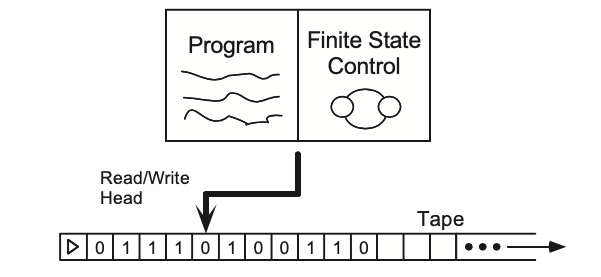
\includegraphics[width=0.70\textwidth]{turing.png}
    \caption{Main elements of a Turing machine}
\end{figure}
\vspace{1em}

The finite state control for a Turing machine consists of a finite set of internal states, $q_1,\dots, q_m$. The number $m$ is allowed to be varied; it turns out that for $m$ sufficiently large this does not affect the power of the machine in any essential way, so without loss of generality we may suppose that $m$ is some fixed constant. The best way to think of the finite state control is as a sort of microprocessor, coordinating the Turing machine’s operation. It provides temporary storage off-tape, and a central place where all processing for the machine may be done. In addition to the states $q_1 , \dots , q_m$ , there are also two special internal states, labelled $q_s$ and $q_h$. We call these the starting state and the halting state, respectively. The idea is that at the beginning of the computation, the Turing machine is in the starting state $q_s$. The execution of the computation causes the Turing machine’s internal state to change. If the computation ever finishes, the Turing machine ends up in the state $q_h$ to indicate that the machine has completed its operation.
\vspace{1em}

The Turing machine tape is a one-dimensional object, which stretches off to infinity in one direction. The tape consists of an infinite sequence of tape squares. We number the tape squares $0,1,2,3,\dots$ The tape squares each contain one symbol drawn from some alphabet, $\Gamma$, which contains a finite number of distinct symbols. For now, it will be convenient to assume that the alphabet contains four symbols, which we denote by $0, 1, b$ (the ‘blank’ symbol), and an arrow, to mark the left hand edge of the tape. Initially, the tape contains an arrow at the left hand end, a finite number of $0s$ and $1s$, and the rest of the tape contains blanks. The read-write tape-head identifies a single square on the Turing machine tape as the square that is currently being accessed by the machine.
\vspace{1em}

A \textit{program} for a Turing machine is a finite ordered list of program lines of the form $\langle q, x, q', x', s\rangle$. The first item in the program line, $q$, is a state from the set of internal states of the machine. The second item, $x$, is taken from the alphabet of symbols which may appear on the tape, $\Gamma$. The way the program works is that on each machine cycle, the Turing machine looks through the list of program lines in order, searching for a line $\langle q, x, \cdot, \cdot, \cdot \rangle$, such that the current internal state of the machine is $q$, and the symbol being read on the tape is $x$. If it doesn't find such a program line, the internal state of the machine is changed to $q_h$, and the machine halts operation. If such a line is found, then that program line is executed. Execution of a program line involves the following steps: the internal state of the machine is changed to $q'$; the symbol $x$ on the tape is overwritten by the symbol $x'$, and the tape-head moves left, right, or stands still, depending on whether $s$ is $-1$, $+1$, or $0$, respectively. The only exception to this rule is if the tape-head is at the leftmost tape square, and $s = -1$, in which case the tape-head stays put.
\vspace{1em}

It turns out that the Turing machine model of computation can be used to compute an enormous variety of functions. For example, it can be used to do all the basic arithmetical operations, to search through text represented as strings of bits on the tape, and many other interesting operations. Surprisingly, it turns out that a Turing machine can be used to simulate all the operations performed on a modern computer! Indeed, according to a thesis put forward independently by Church and by Turing, the Turing machine model of computation completely captures the notion of computing a function using an algorithm. This is known as the Church–Turing thesis:
\textit{The class of functions computable by a Turing machine corresponds exactly to the class of functions which we would naturally regard as being computable by an algorithm.}

\subsubsection*{The Universal Turing Machine}
We've described Turing machines as containing three elements which may vary from machine to machine - the initial configuration of the tape, the internal states of the finite state control, and the program for the machine. A clever idea known as the Universal Turing Machine (UTM) allows us to fix the program and finite state control once and for all, leaving the initial contents of the tape as the only part of the machine which needs to be varied.
The Universal Turing Machine (see the figure below) has the following property. Let $M$ be any Turing machine, and let $T_M$ be the Turing number associated to machine $M$. Then on input of the binary representation for $T_M$ followed by a blank, followed by any string of symbols $x$ on the remainder of the tape, the Universal Turing Machine gives as output whatever machine $M$ would have on input of $x$. Thus, the Universal Turing Machine is capable of simulating any other Turing machine!

\begin{figure}[h]
    \centering
    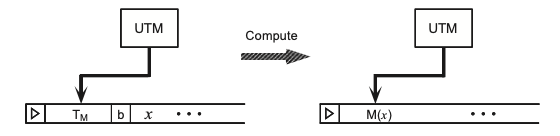
\includegraphics[width=0.70\textwidth]{UTM.png}
\end{figure}
\vspace{1em}

\subsection{Circuits}
Turing machines are rather idealized models of computing devices. Real computers are finite in size, whereas for Turing machines we assumed a computer of unbounded size. Here we investigate an alternative model of computation, the circuit model, that is equivalent to the Turing machine in terms of computational power, but is more convenient and realistic for many applications. In particular the circuit model of computation is especially important as preparation for our investigation of quantum computers.
\vspace{1em}

A circuit is made up of \textit{wires} and \textit{gates}, which carry information around, and perform simple computational tasks, respectively. More generally, a circuit may involve many input and output bits, many wires, and many logical gates. A \textit{logic gate} is a function $f : \{0,1\}^k \rightarrow \{0,1\}^l$ from some fixed number $k$ of input bits to some fixed number $l$ of output bits. 
\vspace{1em}

The following figure shows the circuit representation of the elementary logic gates.

\begin{figure}[h]
    \centering
    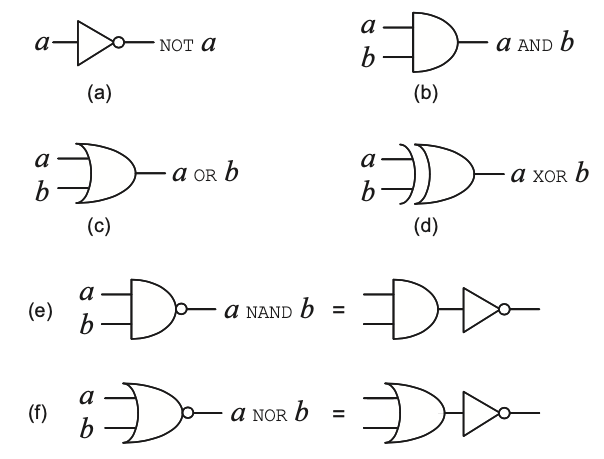
\includegraphics[width=0.70\textwidth]{logic_gates.png}
\end{figure}
\vspace{1em}

Now, let’s look at a simple example of a circuit which adds two $n$ bit integers. The basic element in this circuit is a smaller circuit known as a half-adder. A half-adder takes two bits, $x$ and $y$, as input, and outputs the sum of the bits $x \oplus y$ modulo $2$, together with a carry bit set to $1$ if $x$ and $y$ are both $1$, or $0$ otherwise.
\begin{figure}[h]
    \centering
    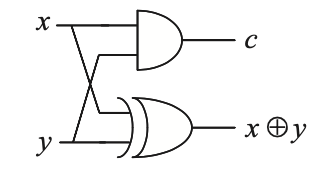
\includegraphics[width=0.35\textwidth]{half_adder.png}
    \caption{Half-adder circuit}
\end{figure}
\vspace{1em}

Two cascaded half-adders may be used to build a full-adder, as shown in the following figure. A full-adder takes as input three bits, $x$, $y$, and $c$. The bits $x$ and $y$ should be thought of as data to be added, while $c$ is a carry bit from an earlier computation. The circuit outputs two bits. One output bit is the modulo $2$ sum, $x \oplus y \oplus c$ of all three input bits. The second output bit, $c'$, is a carry bit, which is set to $1$ if two or more of the inputs is $1$, and is $0$ otherwise.
\begin{figure}[h]
    \centering
    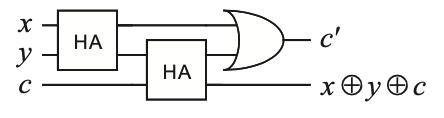
\includegraphics[width=0.55\textwidth]{full_adder.png}
    \caption{Full-adder circuit}
\end{figure}
\vspace{1em}

By cascading many of these full-adders together we obtain a circuit to add two $n$-bit
integers, as illustrated in the figure for the case $n = 3$.
\begin{figure}[h]
    \centering
    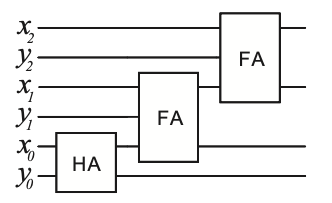
\includegraphics[width=0.45\textwidth]{3_adder.png}
    \caption{Addition circuit for two three-bit integers}
\end{figure}
\vspace{1em}

We claimed earlier that just a few fixed gates can be used to compute any function $f : \{0, 1\}^n \rightarrow \{0, 1\}^m$ whatsoever. We will now prove this for the simplified case of a function $f : \{0, 1\}^n \rightarrow \{0, 1\}$ with $n$ input bits and a single output bit. Such a function is known as a \textit{Boolean function}, and the corresponding circuit is a \textit{Boolean circuit}. The general universality proof follows immediately from the special case of Boolean functions. The proof is by induction on $n$. For $n = 1$ there are four possible functions: the identity, which has a circuit consisting of a single wire; the bit flip, which is implemented using a single $NOT$ gate; the function which replaces the input bit with a $0$, which can be obtained by $AND$ing the input with a work bit initially in the $0$ state; and the function which replaces the input with a $1$, which can be obtained by $OR$ing the input with a work bit initially in the $1$ state.
\vspace{1em}

To complete the induction, suppose that any function on $n$ bits may be computed by a circuit, and let $f$ be a function on $n + 1$ bits. Define n-bit functions $f_0$ and $f_1$ by $f_0(x_1,\dots,x_n) \equiv f(0,x_1,\dots,x_n)$ and $f_1(x_1,\dots,x_n) \equiv f(1,x_1,\dots,x_n)$. These are both $n$-bit functions, so by the inductive hypothesis there are circuits to compute these functions.
\vspace{1em}

It is now an easy matter to design a circuit which computes $f$. The circuit computes both $f_0$ and $f_1$ on the last $n$ bits of the input. Then, depending on whether the first bit of the input was a $0$ or a $1$ it outputs the appropriate answer. A circuit to do this is shown in the following figure. This completes the induction.
\begin{figure}[h]
    \centering
    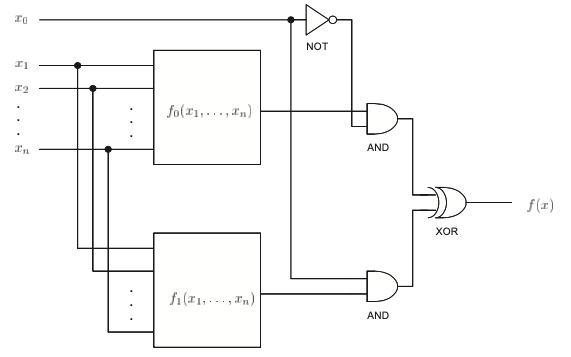
\includegraphics[width=0.70\textwidth]{induction.png}
    \caption{Circuit to compute an arbitrary function $f$ on $n + 1$ bits, assuming by induction that there are circuits to compute the $n$-bit functions $f_0$ and $f_1$.}
\end{figure}

\newpage
Let’s return from our brief quantum digression, to the properties of classical circuits. We claimed earlier that the Turing machine model is equivalent to the circuit model of computation. In what sense do we mean the two models are equivalent? On the face of it, the two models appear quite different. The unbounded nature of a Turing machine makes them more useful for abstractly specifying what it is we mean by an algorithm, while circuits more closely capture what an actual physical computer does.
\vspace{1em}

The two models are connected by introducing the notion of a \textit{uniform circuit family}. A circuit family consists of a collection of circuits, $\{C_n\}$, indexed by a positive integer $n$. The circuit $C_n$ has $n$ input bits, and may have any finite number of extra work bits, and output bits. The output of the circuit $C_n$, upon input of a number $x$ of at most $n$ bits in length, is denoted by $C_n(x)$. We require that the circuits be consistent, that is, if $m \lt n$ and $x$ is at most $m$ bits in length, then $C_m(x) = C_n(x)$. The function computed by the circuit family $\{C_n\}$ is the function $C(\cdot)$ such that if $x$ is $n$ bits in length then $C(x) = C_n(x)$. For example, consider a circuit $C_n$ that squares an $n$-bit number. This defines a family of circuits ${C_n}$ that computes the function, $C(x) = x^2$, where $x$ is any positive integer.
\vspace{1em}

In this section we saw the two models of computation and realized that the circuit model is a realistic one. In the next section we will learn about quantum circuits which are at the heart of realizing a quantum computer.
\newpage
\section{Quantum circuits}

In the previous chapter, we discussed the classical models of computation including classical circuits. In this chapter, we will discuss about the quantum circuits which lie at the heart of quantum computation. There are two main ideas introduced in this chapter. First, we explain in detail the fundamental model of quantum computation, the quantum circuit model. Second, we demonstrate that there exists a small set of gates which are \textit{universal}, that is, any quantum computation whatsoever can be expressed in terms of those gates.

\subsection{Single qubit operations}

As we have already seen previously that a qubit is a vector $\ket{\psi} = a\ket{0} + b\ket{1}$ parameterized by two complex numbers satisfying $|a|^2 + |b|^2 = 1$. Operations on a qubit must preserve this norm, and thus are described by $2 \times 2$ unitary matrices. It should be noted that \textit{all} unitary matrices are valid gates for a qubit. Here are some commonly used single qubit gates: 
\begin{figure}[h]
    \centering
    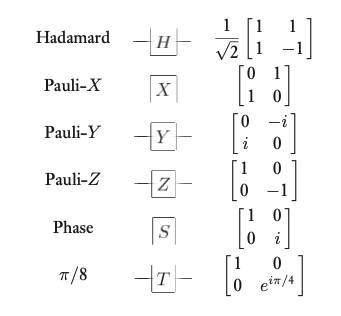
\includegraphics[width=0.45\textwidth]{gates.png}
    \caption{Names, symbols, and unitary matrices for the common single qubit gates.}
\end{figure}
\vspace{1em}

\subsection{Controlled operations}

'If A is true, then do B'. This type of \textit{controlled operation} is one of the most useful in computing, both classical and quantum.
\vspace{1em}

Suppose we have a single qubit gate $U$. A \textit{Controlled-$U$} gate is a two qubit gate which takes in an extra qubit called control qubit which is either $\ket{0}$ or $\ket{1}$. If it is $\ket{1}$, then the gate $U$ is applied on the other qubit (target qubit). However, if it is $\ket{0}$, then the other qubit is not changed. Mathematically, $\ket{c}\ket{t} \rightarrow \ket{c}U^c\ket{t}$ where $U^c = U$ if $c = \ket{1}$ and $U^c = I$ if $c = \ket{0}$. It is represented as follows.
\begin{figure}[h]
    \centering
    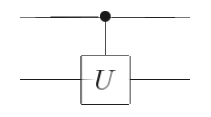
\includegraphics[width=0.20\textwidth]{controlled.png}
    \caption{Controlled-$U$ operation}
\end{figure}
\vspace{1em}

If $U$ is the NOT gate, then we get what is called the CNOT gate. It is a very useful gate as we will see later and has the following matrix representation.

$$\begin{bmatrix}
1&0&0&0\\
0&1&0&0\\
0&0&0&1\\
0&0&1&0\\
\end{bmatrix}$$
\vspace{1em}

The advantage of CNOT gate that any general controlled-$U$ gate can easily be derived CNOT gate by using the circuit given below.
\begin{figure}[h]
    \centering
    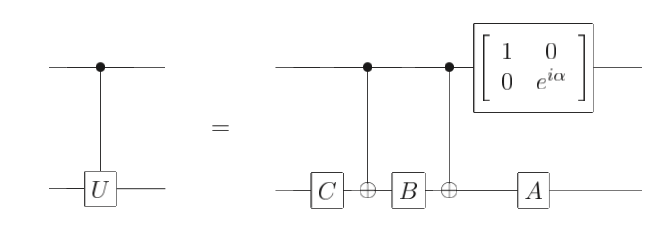
\includegraphics[width=0.70\textwidth]{cu.png}
    \caption{Circuit implementing the controlled-$U$ operation for single qubit gate $U$. $\alpha$, $A$, $B$ and $C$ satisfy $U = e^{i\alpha}A\times B\times C$, $ABC = I$.}
\end{figure}
\vspace{1em}

\subsection{Measurement}

A final element used in quantum circuits, almost implicitly sometimes, is measurement. In circuit diagrams, a measurement is reresented using the 'meter' symbol. In the theory of quantum circuits it is conventional to not use any special symbols to denote more general measurements, because they can always be represented by unitary transforms with ancilla qubits followed by projective measurements.
\vspace{1em}
\begin{figure}[h]
    \centering
    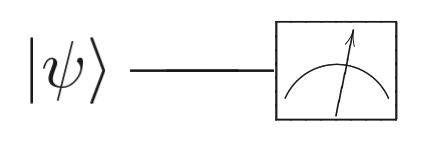
\includegraphics[width=0.40\textwidth]{meter.png}
    \caption{Symbol for measurement on a single qubit.}
\end{figure}
\vspace{1em}

There are two important principles that it is worth bearing in mind about quantum circuits.

\begin{enumerate}
    \item\textbf{Principle of deferred measurement}: Measurements can always be moved from an intermediate stage of a quantum circuit to the end of the circuit; if the measurement results are used at any stage of the circuit then the classically controlled operations can be replaced by conditional quantum operations.
    \item\textbf{Principle of implicit measurement}: Without loss of generality, any unterminated quantum wires (qubits which are not measured) at the end of a quantum circuit may be assumed to be measured.
\end{enumerate}

\subsection{Universal quantum gates}

A set of gates is said to be universal for quantum computation if any unitary operation may be approximated to arbitrary accuracy by a quantum circuit involving only those gates.
\vspace{1em}

We now describe three universality constructions for quantum computation.

\subsubsection{Two-level unitary gates are universal}

Consider a unitary matrix $U$ which acts on a $d$-dimensional Hilbert space. In this section we explain how $U$ may be decomposed into a product of two-level unitary matrices; that is, unitary matrices which act non-trivially only on two-or-fewer vector components. The essential idea behind this decomposition may be understood by considering the case when $U$ is $3\times 3$, so suppose that $U$ has the form
$$U = \begin{bmatrix}
a&d&g\\
b&e&h\\
c&f&j
\end{bmatrix}$$

We will find two-level unitary matrices $U_1, U_2, U_3$ such that
$$U_3U_2U_1U = I$$
It follows that
$$U = U_1^\dag U_2^\dag U_3^\dag$$

$U_1$, $U_2$ and $U_3$ are all two-level unitary matrices, and it is easy to see that their inverses, $U_1^\dag$, $U_2^\dag$ and $U_3^\dag$ are also two-level unitary matrices.
\vspace{1em}

Use the following procedure to construct $U_1$: if $b = 0$ then set
$$U_1 \equiv \begin{bmatrix}1&0&0\\0&1&0\\0&0&1\end{bmatrix}$$
If $b \neq 0$ then set
$$U_1 \equiv \begin{bmatrix}
\frac{a^\ast}{\sqrt{|a|^2+|b|^2}} & \frac{b^\ast}{\sqrt{|a|^2+|b|^2}} &0\\
\frac{b}{\sqrt{|a|^2+|b|^2}} & \frac{-a}{\sqrt{|a|^2+|b|^2}} &0\\
0&0&1
\end{bmatrix}$$

Note that in either case $U_1$ is a two-level unitary matrix, and when we multiply the matrices out we get
$$U_1U = \begin{bmatrix}
a'&d'&g'\\
0&e'&h'\\
c'&f'&j'
\end{bmatrix}$$

The key point to note is that the middle entry in the left hand column is zero. Now apply a similar procedure to find a two-level matrix $U_2$ such that $U_2U_1U$ has no entry in the bottom left corner. That is, if $c' = 0$ we set
$$U_2 \equiv \begin{bmatrix}a'^\ast&0&0\\0&1&0\\0&0&1\end{bmatrix}$$
while if $c' \neq 0$ then we set
$$U_2 \equiv \begin{bmatrix}
\frac{a'^\ast}{\sqrt{|a'|^2+|c'|^2}} &0& \frac{a'^\ast}{\sqrt{|a'|^2+|c'|^2}}\\
0&1&0\\
\frac{c'}{\sqrt{|a'|^2+|c'|^2}} &0& \frac{-a'}{\sqrt{|a'|^2+|c'|^2}}
\end{bmatrix}$$
In either case, when we carry out the matrix multiplication we find that
$$U_2U_1U = \begin{bmatrix}
1&d''&g''\\
0&e''&h''\\
0&f''&j''
\end{bmatrix}$$
Since $U$, $U_1$ and $U_2$ are unitary, it follows that $U_2U_1U$ is unitary, and thus $d'' = g'' = 0$ since the first row of $U_2U_1U$ must have norm $1$. Finally, set
$$U_3 = \begin{bmatrix}
1&0&0\\
0&e''^\ast&h''^\ast\\
0&f''^\ast&j''^\ast
\end{bmatrix}$$
It is now easy to verify that $U_3U_2U_1U = I$, and thus $U = U_1^\dag U_2^\dag U_3^\dag$, which is a decomposition of $U$ into two-level unitaries.
\vspace{1em}

More generally, suppose $U$ acts on a $d$-dimensional space. Then, in a similar fashion to the $3\times 3$ case, we can find two-level unitary matrices $U_1, \dots , U_{d-1}$ such that the matrix $U_{d-1}U_{d-2}\dots U_1U$ has a one in the top left hand corner, and all zeroes elsewhere in the first row and column. We then repeat this procedure for the $d - 1$ by $d - 1$ unitary submatrix in the lower right hand corner of $U_{d-1}U_{d-2}\dots U_1U$ , and so on, with the end result that an arbitrary $d\times d$ unitary matrix may be written
$$U = V_1\dots V_k$$
where the matrices $V_i$ are two-level unitary matrices, and $k \leq (d - 1) + (d - 2) + \dots + 1 = d(d-1)/2$.

\subsubsection{Single qubit and CNOT gates are universal}

Suppose $U$ is a two-level unitary matrix on an $n$ qubit quantum computer. Suppose
in particular that $U$ acts non-trivially on the space spanned by the computational basis
states $\ket{s}$ and $\ket{t}$, where $s = s_1\dots s_n$ and $t = t_1\dots t_n$ are the binary expansions for $s$ and $t$. Let $\widetilde{U}$ be the non-trivial $2\times 2$ unitary submatrix of $U$; $\widetilde{U}$ can be thought of as a unitary operator on a single qubit.
\vspace{1em}

Our immediate goal is to construct a circuit implementing $U$, built from single qubit and CNOT gates. To do this, we need to make use of \textit{Gray codes}. Suppose we have distinct binary numbers, $s$ and $t$. A Gray code connecting $s$ and $t$ is a sequence of binary numbers, starting with $s$ and concluding with $t$, such that adjacent members of the list differ in exactly one bit. For instance, with $s = 101001$ and $t = 110011$ we have the Gray code
$$\begin{matrix}1&0&1&0&0&1\\1&0&1&0&1&1\\1&0&0&0&1&1\\1&1&0&0&1&1\end{matrix}$$

Let $g_1$ through gm be the elements of a Gray code connecting $s$ and $t$, with $g_1 = s$ and $g_m = t$. Note that we can always find a Gray code such that $m \le n+1$ since $s$ and $t$ can differ in at most $n$ locations.
\vspace{1em}

Now, the first step is to swap the states $\ket{g_1}$ and $\ket{g_2}$. Suppose $g_1$ and $g_2$ differ at the $i$th digit. Then we accomplish the swap by performing a controlled bit flip on the $i$th qubit, conditional on the values of the other qubits being identical to those in both $g_1$ and $g_2$. Next we use a controlled operation to swap $\ket{g_2}$ and $\ket{g_3}$. We continue in this fashion until we swap $\ket{g_{m-2}}$ with $\ket{g_{m-1}}$. The effect of this sequence of $m − 2$ operations is to achieve the operation
\begin{equation*}
\begin{split}
    \ket{g_1} &\rightarrow \ket{g_{m-1}}\\
    \ket{g_2} &\rightarrow \ket{g_1}\\
    \ket{g_3} &\rightarrow \ket{g_2}\\
    &\dots\\
    \ket{g_{m-1}} &\rightarrow \ket{g_{m-2}}
\end{split}
\end{equation*}

All other computational basis states are left unchanged by this sequence of operations.
Next, suppose $g_{m−1}$ and $g_m$ differ in the $j$th bit. We apply a controlled-$\widetilde{U}$ operation with the $j$th qubit as target, conditional on the other qubits having the same values as appear in both $g_m$ and $g_{m−1}$. Finally, we complete the $U$ operation by undoing the swap operations: we swap $\ket{g_{m-1}}$ with $\ket{g_{m-2}}$, then $\ket{g_{m-2}}$ with $\ket{g_{m-3}}$ and so on, until we swap $\ket{g_2}$ with $\ket{g_1}$.
\vspace{1em}

We see that implementing the two-level unitary operation $U$ requires at most $2(n−1)$ controlled operations to swap $\ket{g_1}$ with $\ket{g_{m-1}}$ and then back
again. Each of these controlled operations can be realized using $O(n)$ single qubit and CNOT gates; the controlled-$\widetilde{U}$ operation also requires $O(n)$ gates. Thus, implementing $U$ requires $O(n^2)$ single qubit and CNOT gates. We saw in the previous section that an arbitrary unitary matrix on the $2n$-dimensional state space of $n$ qubits may be written as a product of $O(2^{2n}) = O(4^n)$ two-level unitary operations. Combining these results, we see that an arbitrary unitary operation on $n$ qubits can be implemented using a circuit containing $O(n^2 4^n)$ single qubit and CNOT gates. 

\newpage
\section{The quantum Fourier transform and its applications}

In the introduction, we stated that quantum computers can factor numbers much faster than a classical computer. To put this in perspective, finding the prime factorization of an $n$-bit integer is thought to require $exp(O(n^{1/3}\log^{2/3}n))$ operations using the best classical algorithm known, the so-called number \textit{field sieve}. In contrast, a quantum algorithm can accomplish the same task using $O(n^2 \log n \log\log n)$ operations. That is, a quantum computer can factor a number \textit{exponentially} faster than the best known classical algorithms.
\vspace{1em}

But now the question arises, what other tasks a quantum computer can do more efficiently than a classical computer? In this chapter, we talk about the \textit{quantum Fourier transform} which is the key ingredient for quantum factoring and many other interesting quantum algorithms.

\subsection{The quantum Fourier transform}

A very useful and common way to solve a problem in computer science is to break it down or \textit{transform} it into other problem(s) whose solution is known. A great discovery of quantum computation has been that some such transformations can be computed much faster on a quantum computer than on a classical computer.
\vspace{1em}

One such transformation is the discrete Fourier transform. In the usual mathematical notation, the discrete Fourier transform takes as input a vector of complex numbers, $x_0 , \dots , x_{N-1}$ where the length $N$ of the vector is a fixed parameter. It outputs the transformed data, a vector of complex numbers $y_0,\dots,y_{N−1}$, defined by
$$y_k \equiv \frac{1}{\sqrt{N}}\sum_{j=0}^{N-1}{x_j e^{2\pi ijk/N}}$$

The quantum Fourier transform is exactly the same transformation, although the conventional notation for the quantum Fourier transform is somewhat different. The quantum Fourier transform on an orthonormal basis $\ket{0},\dots, \ket{N - 1}$ is defined to be a linear operator with the following action on the basis states,
$$\ket{j} \rightarrow \frac{1}{\sqrt{N}}\sum_{j=0}^{N-1}{e^{2\pi ijk/N}\ket{k}}$$

Equivalently, the action on an arbitrary state may be written
$$\sum_{j=0}^{N-1}{x_j\ket{j}} \rightarrow \sum_{k=0}^{N-1}{y_k\ket{k}},$$
where the amplitudes $y_k$ are the discrete Fourier transform of the amplitudes $x_j$. Now we shall demonstrate the unitarity of the Fourier transform by constructing a manifestly unitary quantum circuit computing the Fourier transform.
\vspace{1em}

In the following, we take $N = 2^n$, where n is some integer, and the basis $\ket{0},\dots , \ket{2^n-1}$ is the computational basis for an $n$ qubit quantum computer. It is helpful to write the state $\ket{j}$ using the binary representation $j = j_1j_2\dots j_n$. More formally, $j = j_1 2^n−1 + j_2 2^n−2 + \dots + j_n 2^0$ . It is also convenient to adopt the notation $0.j_lj_{l+1}\dots j_m$ to represent the binary fraction $j_l/2 + j_{l+1}/4 + \dots + j_m/2^{m-l+1}$.
\vspace{1em}

With a little algebra the quantum Fourier transform can be given the following useful \textit{product representation}:
$$\ket{j_1,\dots,j_n} \rightarrow \ddfrac{\Big(\ket{0} + e^{2\pi i0.j_n}\ket{1}\Big)\Big(\ket{0} + e^{2\pi i0.j_{n-1}j_n}\ket{1}\Big)\dots\Big(\ket{0} + e^{2\pi i0.j_1j_2\dots j_n}\ket{1}\Big)}{2^{n/2}}$$

\newpage
The equivalence of the product representation and the definition follows from some elementary algebra:
\begin{equation*}
\begin{split}
    \ket{j} & \rightarrow \frac{1}{2^{n/2}}\sum_{k=0}{2^n-1}{e^{2\pi ijk/2^n}\ket{k}}\\
    & = \frac{1}{2^{n/2}} \sum_{k_1=0}^{1}\dots\sum_{k_n=0}^{1}{e^{2\pi ij\big(\sum_{l=1}^{n}{k_l2^{-l}}\big)}\ket{k_1\dots k_n}}\\
    & = \frac{1}{2^{n/2}} \sum_{k_1=0}^{1}\dots\sum_{k_n=0}^{1}{\bigotimes_{l=1}^{n}{e^{2\pi ijk_l2^{-l}}\ket{k_l}}}\\
    & = \frac{1}{2^{n/2}} \bigotimes_{l=1}^{n}{\Bigg[\sum_{k_l=0}{1}{e^{2\pi ijk_l2^{-l}}\ket{k_l}}\Bigg]}\\
    & = \frac{1}{2^{n/2}} \bigotimes_{l=1}^{n}{\bigg[\ket{0} + e^{2\pi ij2^{-l}}\ket{1}\bigg]}\\
    & = \ddfrac{\Big(\ket{0} + e^{2\pi i0.j_n}\ket{1}\Big)\Big(\ket{0} + e^{2\pi i0.j_{n-1}j_n}\ket{1}\Big)\dots\Big(\ket{0} + e^{2\pi i0.j_1j_2\dots j_n}\ket{1}\Big)}{2^{n/2}}
\end{split}
\end{equation*}

The product representation makes it easy to derive an efficient circuit for the quantum Fourier transform. Such a circuit is shown in the figure. The gate $R_k$ denotes the unitary transformation
$$R_k \equiv \begin{bmatrix}1&0\\0&e^{2\pi i/2^k}\end{bmatrix}$$
\begin{figure}[h]
    \centering
    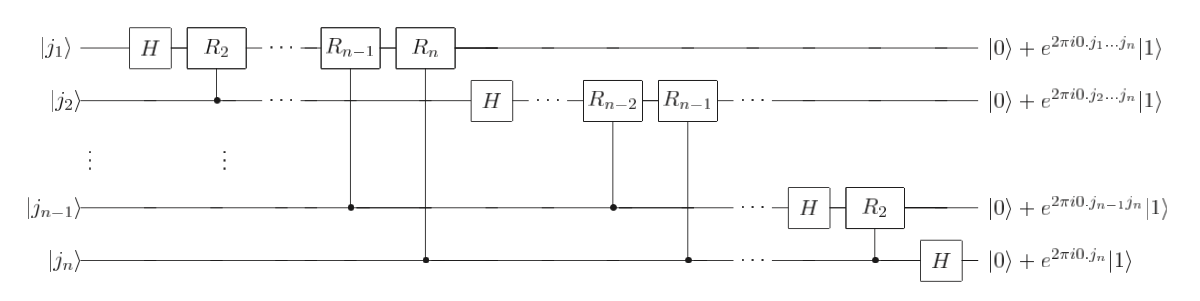
\includegraphics[width=1.0\textwidth]{fourier_circuit.png}
    \caption{Efficient circuit for the quantum Fourier transform.}
\end{figure}

\subsection{Phase estimation}

The Fourier transform is the key to a general procedure known as \textit{phase estimation}, which in turn is the key for many quantum algorithms. Suppose a unitary operator $U$ has an eigenvector $\ket{u}$ with eigenvalue $e^{2\pi i\phi}$, where the value of $\phi$ is unknown. The goal of the phase estimation algorithm is to estimate $\phi$. To do this, we will assume that we already have available some \textit{black boxes} capable of preparing the state $\ket{u}$ and performing the controlled-$U^2^j$ operation, for suitable non-negative integers $j$.
\vspace{1em}

The quantum phase estimation procedure uses two registers. The first register contains $t$ qubits initially in the state $\ket{0}$. How we choose $t$ depends on two things: the number of digits of accuracy we wish to have in our estimate for $\phi$, and with what probability we wish the phase estimation procedure to be successful. The second register begins in the state $\ket{u}$, and contains as many qubits as is necessary to store $\ket{u}$. Phase estimation is performed in two stages. First, we apply the circuit shown in the figure. The circuit begins by applying a Hadamard transform to the first register, followed by application of controlled-$U$ operations on the second register, with $U$ raised to successive powers of two. The final state of the first register is easily seen to be:
$$\frac{1}{2^{t/2}}\Big(\ket{0} + e^{2\pi i2^{t-1}\phi}\ket{1}\Big)\Big(\ket{0} + e^{2\pi i2^{t-2}\phi}\ket{1}\Big)\dots\Big(\ket{0} + e^{2\pi i2^{0}\phi}\ket{1}\Big)
= \frac{1}{2^{t/2}}\sum_{k=0}^{2^t-1}{e^{2\pi i\phi k}\ket{k}}$$
We omit the second register from this description, since it stays in the state $\ket{u}$ throughout the computation.
\begin{figure}[h]
    \centering
    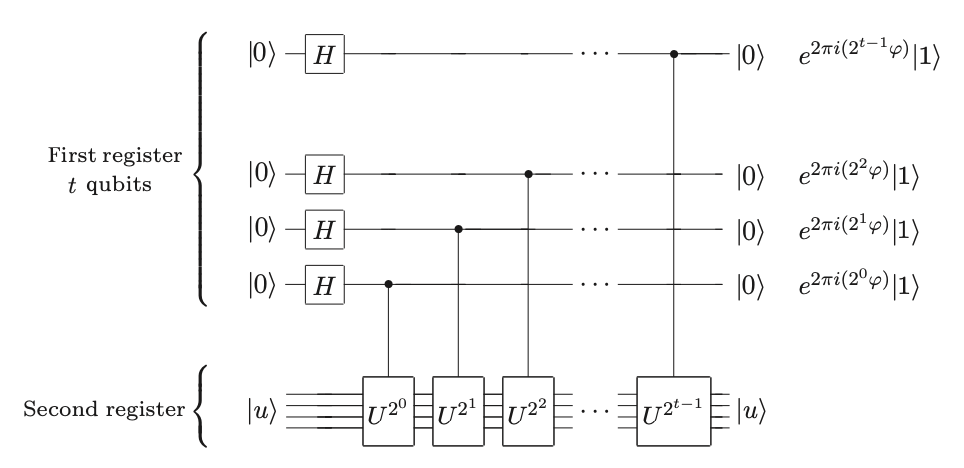
\includegraphics[width=1.0\textwidth]{phase_est.png}
    \caption{The first stage of the phase estimation procedure.}
\end{figure}
\vspace{1em}

The second stage of phase estimation is to apply the inverse quantum Fourier transform on the first register. This is obtained by reversing the circuit for the quantum Fourier transform, and can be done in $\Theta(t^2)$ steps. The third and final stage of phase estimation is to read out the state of the first register by doing a measurement in the computational basis. We will show that this provides a pretty good estimate of $\phi$. An overall schematic of the algorithm is shown below.
\begin{figure}[h]
    \centering
    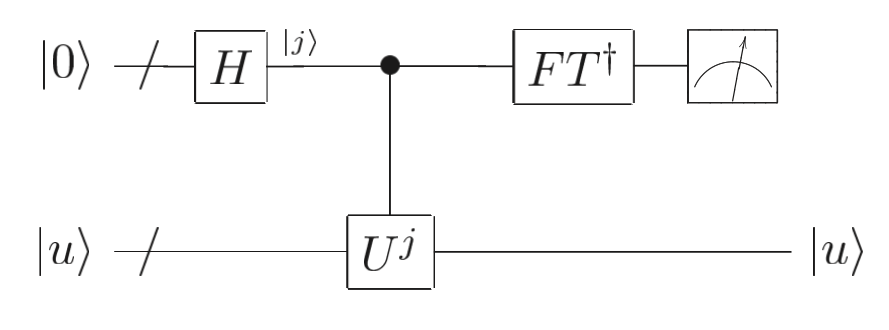
\includegraphics[width=0.8\textwidth]{overall_phase.png}
    \caption{Schematic of the overall phase estimation procedure.}
\end{figure}

\newpage
To see why phase estimation works, suppose $\phi$ may be expressed exactly in $t$ bits, as $\phi = 0.\phi_1\dots\phi_t$. Then the state resulting from the first stage of phase estimation may be rewritten
$$\frac{1}{2^{t/2}}\Big(\ket{0} + e^{2\pi i0.\phi_t}\ket{1}\Big)\Big(\ket{0} + e^{2\pi i0.\phi_{t-1}\phi_t}\ket{1}\Big)\dots\Big(\ket{0} + e^{2\pi i0.\phi_1\dots\phi_t}\ket{1}\Big)$$
The second stage of phase estimation is to apply the inverse quantum Fourier transform. But comparing the previous equation with the product form for the Fourier transform, we see that the output state from the second stage is the product state $\ket{\phi_1\dots\phi_t}$. A measurement in the computational basis therefore gives us $\phi$ exactly!

\subsection{Applications}

\subsubsection{Application: order-finding}

For positive integers $x$ and $N$ , $x < N$ , with no common factors, the \textit{order} of $x$ modulo $N$ is defined to be the least positive integer, $r$, such that $x^r = 1\ (mod\ N)$. The order-finding problem is to determine the order for some specified $x$ and $N$. Order-finding is believed to be a hard problem on a classical computer, in the sense that no algorithm is known to solve the problem using resources polynomial in the $O(L)$ bits needed to specify the problem, where $L \equiv \lceil\log(N)\rceil$ is the number of bits needed to specify $N$. In this section we explain how phase estimation may be used to obtain an efficient quantum algorithm for order-finding.
\vspace{1em}

The quantum algorithm for order-finding is just the phase estimation algorithm applied to the unitary operator
$$U\ket{y} \equiv \ket{xy\ (mod\ N)}$$
A simple calculation shows that the states defined by
$$\ket{u_s} \equiv \frac{1}{\sqrt{r}}\sum_{k=0}^{r-1}{\exp{\frac{-2\pi isk}{r}}\ket{x^k\ mod N}},$$
for integer $0 \le s \le r - 1$ are eigenstates of $U$, since
\begin{equation*}
\begin{split}
    U\ket{u_s} & = \frac{1}{\sqrt{r}}\sum_{k=0}^{r-1}{\exp{\frac{-2\pi isk}{r}}\ket{x^{k+1}\ mod N}}\\
    & = \exp{\frac{2\pi is}{r}}\ket{u_s}
\end{split}
\end{equation*}

Using the phase estimation procedure allows us to obtain, with high accuracy, the corresponding eigenvalues $\exp(2\pi is/r)$, from which we can obtain the order $r$ with a little bit more work.

\begin{figure}[h]
    \centering
    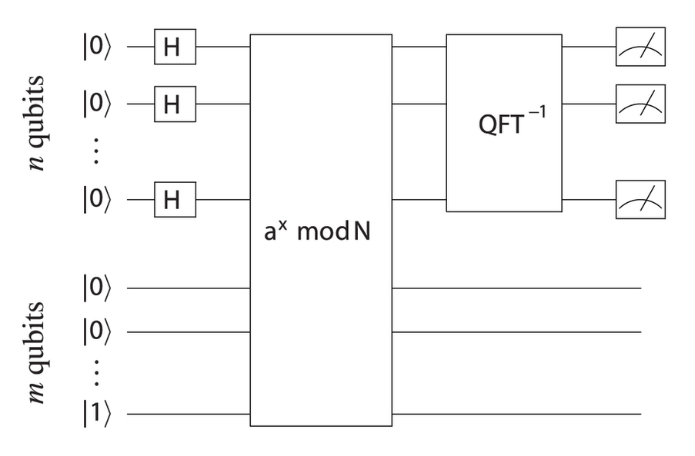
\includegraphics[width=0.8\textwidth]{order_finding.png}
    \caption{Circuit diagram for order finding algorithm.}
\end{figure}

\subsubsection{Application: factoring}

The \textit{factoring problem} goes as follows : given any integer $N$, find all of its prime factors and the exponent with which they appear. This factoring problem turns out to be equivalent to the order-finding problem in the sense that a fast algorithm for order-finding can easily be turned into a fast algorithm for factoring.
\vspace{1em}

The reduction of factoring to order-finding proceeds in two basic steps. The first step is to show that we can compute a factor of $N$ if we can find a non-trivial solution $x \neq \pm 1\ (mod\ N)$ to the equation $x^2 = 1\ (mod\ N)$. The second step is to show that a randomly chosen $y$ co-prime to N is quite likely to have an order $r$ which is even, and such that $y^{r/2} \neq \pm 1\ (mod\ N)$, and thus $x \equiv y^{r/2}\ (mod\ N)$ is a non-trivial solution to $x^2 = 1\ (mod\ N)$.

\begin{theorem}
    Suppose $N$ is an $L$ bit composite number, and $x$ is a non-trivial solution to the equation $x^2 = 1\ (mod\ N)$ in the range $1 \le x \le N$, that is, neither $x = 1\ (mod\ N)$ nor $x = N - 1 = -1\ (mod\ N)$. Then at least one of $\gcd(x - 1,N)$ and $\gcd(x + 1,N)$ is a non-trivial factor of $N$ that can be computed using $O(L^3)$ operations.
\end{theorem}
\begin{theorem}
    Suppose $N = p_1^{\alpha 1}\dots p_m^{\alpha_m}$ is the prime factorization of an odd composite positive integer. Let $x$ be an integer chosen uniformly at random, subject to the requirements that $1 \le x \le N - 1$ and $x$ is co-prime to $N$. Let $r$ be the order of $x$ modulo $N$. Then
    $$p(r\textnormal{ is even and }x^{r/2} \neq -1\ (mod\ N)) \geq 1 - \frac{1}{2^m}$$
\end{theorem}

Above theorems can be combined to give an algorithm which, with high probability, returns a non-trivial factor of any composite $N$. All the steps in the algorithm can be performed efficiently on a classical computer except (so far as is known today) an order-finding 'subroutine' which is used by the algorithm. By repeating the procedure we may find a complete prime factorization of $N$. The algorithm is summarized below.
\vspace{1em}

\textbf{Algorithm: Reduction of factoring to order-finding}
\begin{quote}
    \textbf{Inputs:} A composite number $N$.\\
    \textbf{Outputs:} A non-trivial factor of $N$.\\
    \textbf{Runtime:} $O((\log N)^3)$ operations. Succeeds with probability $O(1)$.\\
    \textbf{Procedure:}
    \begin{enumerate}
        \item If $N$ is even, return the factor $2$.
        \item Determine whether $N = a^b$ for integers $a \geq 1$ and $b \geq 2$, and if so return the factor $a$.
        \item Randomly choose $x$ in the range $1$ to $N-1$. If $\gcd(x,N) > 1$ then return the factor $\gcd(x,N)$.
        \item Use the order-finding subroutine to find the order $r$ of $x$ modulo $N$.
        \item If $r$ is even and $x^{r/2} \neq -1\ (mod\ N)$ then compute $\gcd(x^{r/2}-1,N)$ and $\gcd(x^{r/2} + 1, N)$, and test to see if one of these is a non-trivial factor, returning that factor if so. Otherwise, the algorithm fails.
    \end{enumerate}
\end{quote}

\newpage
\subsubsection{Application : Period-finding}

Consider the following problem. Suppose $f$ is a periodic function producing a single bit as output and such that $f(x + r) = f(x)$, for some unknown $0 < r < 2L$, where $x, r \in \{0, 1, 2, \dots\}$. Given a quantum black box $U$ which performs the unitary transform $U\ket{x}\ket{y} \rightarrow \ket{x}\ket{y \oplus f(x)}$ (where $\oplus$ denotes addition modulo $2$) how many black box queries and other operations are required to determine $r$? Note that in practice $U$ operates on a finite domain, whose size is determined by the desired accuracy for $r$. Here is a quantum algorithm which solves this problem using one query, and $O(L^2)$ other operations:\\
\textbf{Algorithm: Period-finding}
\begin{quote}
    \textbf{Inputs:} (1) A black box which performs the operation $U\ket{x}\ket{y} = \ket{x}\ket{y \oplus f(x)}$, (2) a state to store the function evaluation, initialized to $\ket{0}$, and (3) $t = O(L + \log(1/\epsilon))$ qubits initialized to $\ket{0}$.\\
    \textbf{Outputs:} The least integer $r > 0$ such that $f(x + r) = f(x)$.\\
    \textbf{Runtime:} One use of $U$, and $O(L^2)$ operations. Succeeds with probability $O(1)$.\\
    \textbf{Procedure:}
    \begin{figure}[h]
        \centering
        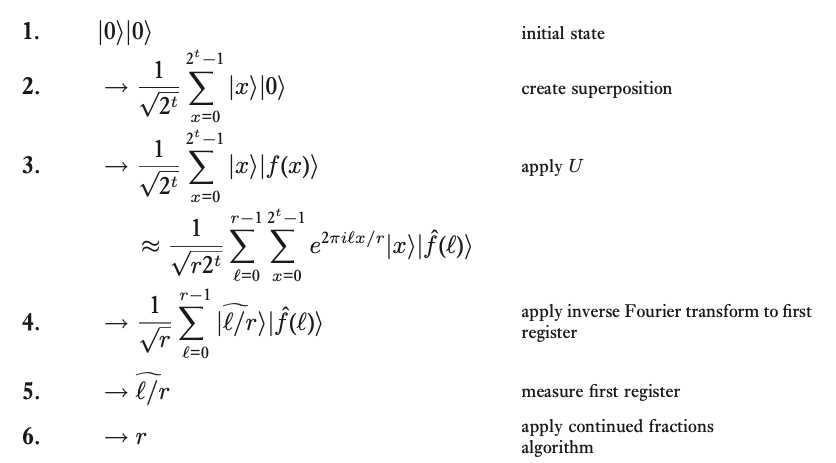
\includegraphics[width=0.9\textwidth]{period_algo.png}
    \end{figure}
\end{quote}
% The circuit diagram for period finding algorithm is as follows.
% \begin{figure}[h]
%     \centering
%     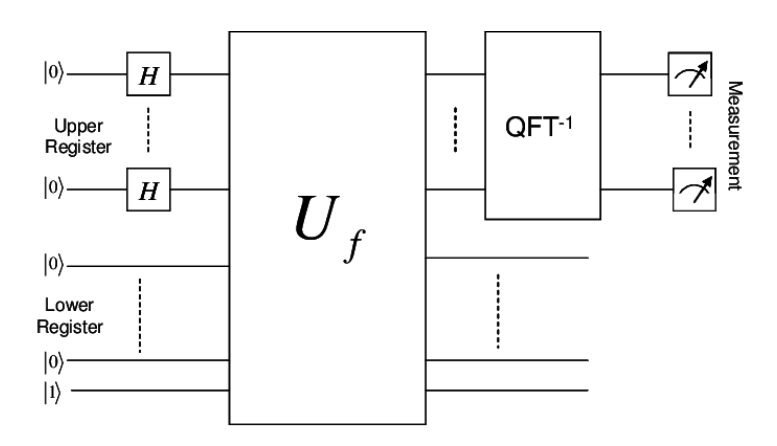
\includegraphics[width=0.8\textwidth]{period_circuit.png}
%     \caption{Circuit diagram for period finding algorithm.}
% \end{figure}
\newpage
\section{Distance measures for quantum information}
\textit{What does it mean to say that two items of information are similar? What does it mean to say that information is preserved by some process?} These questions are central to a theory of quantum information processing, and the purpose of this chapter is the development of distance measures giving quantitative answers to these questions. Motivated by our two questions we will be concerned with two broad classes of distance measures, \textit{static measures} and \textit{dynamic measures}. Static measures quantify how close two quantum states are, while dynamic measures quantify how well information has been preserved during a dynamic process.

\subsection{Distance measures for classical information}
One way of quantifying the distance between two strings of bits is the \textit{Hamming distance}, defined to be the number of places at which two bit strings are not equal. For example, the bit strings $00010$ and $10011$ differ in the first and last place, so the Hamming distance between them is two. Unfortunately, the Hamming distance between two objects is simply a matter of labeling, and \textit{a priori} there aren't any labels in the Hilbert space arena of quantum mechanics!
\vspace{1em}

The first measure is the \textit{trace distance,} defined by the equation:
$$D(p_x, q_x) \equiv \frac{1}{2}\sum_x{|p_x-q_x|}$$
This quantity is sometimes known as the $L_1$ distance or \textit{Kolmogorov distance}. The trace distance turns out to be a metric on probability distributions, so the use of the term 'distance' is justified.
\vspace{1em}

A second measure of distance between probability distributions, the \textit{fidelity} of the probability distributions $\{p_x\}$ and $\{q_x\}$, is defined by
$$F(p_x, q_x) \equiv \sum_x{\sqrt{p_x q_x}}$$

The fidelity is a very different way of measuring distance between probability distributions
than is the trace distance. The fidelity is just the inner product between vectors with components $\sqrt{p_x}$ and $\sqrt{q_x}$, which lie on a unit sphere.
\begin{figure}[h]
    \centering
    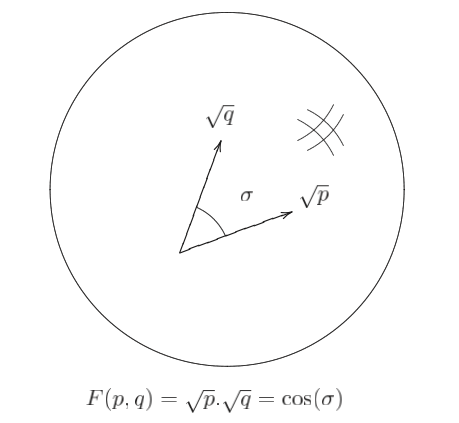
\includegraphics[width=0.4\textwidth]{fidelity.png}
    \caption{Geometric interpretation of the fidelity as the inner product between vectors $\sqrt{p_x}$ and $\sqrt{q_x}$ lying on a unit sphere.}
\end{figure}

\newpage
\subsection{How close are two quantum states?}

\subsubsection{Trace}
Analogous to the classical case, we begin by defining the \textit{trace distance} between quantum states $\rho$ and $\sigma$,
$$D(\rho, \sigma) \equiv \frac{1}{2}\tr|\rho - \sigma|$$
where as per usual we define $|A| \equiv \sqrt{A^\dag A}$ to be the positive square root of $A^\dag A$. Notice that the quantum trace distance generalizes the classical trace distance in the sense that if $\rho$ and $\sigma$ commute then the (quantum) trace distance between $\rho$ and $\sigma$ is equal to the classical trace distance between the eigenvalues of $\rho$ and $\sigma$. More explicitly, if $\rho$ and $\sigma$ commute they are diagonal in the same basis,
$$\rho = \sum_i{r_i\ket{i}\bra{i}};\ \sigma = \sum_i{s_i\ket{i}\bra{i}},$$
for some orthonormal basis $\ket{i}$. Thus
\begin{equation*}
\begin{split}
    D(\rho, \sigma) & = \frac{1}{2}\tr|\sum_i{(r_i - s_i)\ket{i}\bra{i}}|\\
    & = D(r_i, s_i)
\end{split}
\end{equation*}

\begin{theorem}
    Let $\{E_m\}$ be a POVM, with $p_m \equiv \tr(\rho E_m)$ and $q_m \equiv \tr(\sigma E_m)$ as the probabilities of obtaining a measurement outcome labeled by $m$. Then
    $$D(\rho, \sigma) = \max_{\{E_m\}}D(p_m, q_m)$$
    where the maximization is over all POVMs $\{E_m\}$.
\end{theorem}
\begin{proof}
    Note that
    $$D(p_m, q_m) = \frac{1}{2} \sum_m|\tr(E_m(\rho − \sigma))|$$
    Using the spectral decomposition we may write $\rho − \sigma = Q − S$, where $Q$ and $S$ are positive operators with orthogonal support. Thus $|\rho − \sigma| = Q + S$, and
    \begin{equation*}
    \begin{split}
        |tr(E_m(\rho − \sigma))| & = |\tr(E_m(Q - S))|\\
        & \leq |\tr(E_m(Q + S))|\\
        & \leq |\tr(E_m|\rho - \sigma|)|
    \end{split}
    \end{equation*}
    Thus
    \begin{equation*}
    \begin{split}
        D(p_m, q_m) & \leq \frac{1}{2} \sum_m{\tr(E_m|\rho − \sigma|)}\\
        & = \frac{1}{2}\tr|\rho - \sigma|\\
        & = D(\rho, \sigma)
    \end{split}
    \end{equation*}
    where we have applied the completeness relation for POVM elements, $\sum_m{E_m} = I$.\\
    Conversely, by choosing a measurement whose POVM elements include projectors onto the support of $Q$ and $S$, we see that there exist measurements which give rise to probability distributions such that $D(p_m, q_m) = D(\rho, \sigma)$.
\end{proof}

\newpage
\subsubsection{Fidelity}

A second measure of distance between quantum states is the \textit{fidelity}. The fidelity of states $\rho$ and $\sigma$ is defined to be
$$F(\rho,\sigma) ≡ tr\sqrt{\rho^{1/2}\sigma\rho^{1/2}}$$
\begin{theorem}
    \textbf{(Uhlmann’s theorem)} Suppose $\rho$ and $\sigma$ are states of a quantum system $Q$. Introduce a second quantum system $R$ which is a copy of $Q$. Then
    $$F(\rho, \sigma)= max_{\ket{\psi}, \ket{\phi}} |\braket{\psi}{\phi}|$$
    where the maximization is over all purifications $\ket{\psi}$ of $\rho$ and $\ket{\phi}$ of $\sigma$ into $RQ$.
\end{theorem}
\begin{theorem}
    \textbf{(Monotonicity of the fidelity)} Suppose $\mathcal{E}$ is a trace-preserving quantum operation. Let $\rho$ and $\sigma$ be density operators. Show that
    $$F(\mathcal{E}(\rho), \mathcal{E}(\sigma)) \geq F(\rho, \sigma)$$
\end{theorem}
\begin{proof}
    Let $\ket{\psi}$ and $\ket{\phi}$ be purifications of $\rho$ and $\sigma$ into a joint system $RQ$ such that $F(\rho, \sigma) = |\braket{\psi}{\phi}|$. Introduce a model environment $E$ for the quantum operation, $\mathcal{E}$, which starts in a pure state $\ket{0}$, and interacts with the quantum system $Q$ via a unitary interaction $U$. Note that $U\ket{\psi}\ket{0}$ is a purification of $\mathcal{E}\rho$, and $U\ket{\phi}\ket{0}$ is a purification of $\mathcal{E}\sigma$. By Uhlmann's theorem it follows that
    \begin{equation*}
    \begin{split}
        F(\mathcal{E}\rho, \mathcal{E}\sigma) & \geq |\bra{\psi}\bra{0}U^\dag U\ket{\phi}\ket{0}|\\
        & = |\braket{\psi}{\phi}|\\
        & = F(\rho, \sigma)
    \end{split}
    \end{equation*}
\end{proof}
% \newpage
% \section{Revised Plan of Action}
\begin{center}
\begin{tabular}{c|c}
    Week 4 & Density operator, EPR and Bell Inequality, models for computation \\
    Week 5 & Composite quantum systems, quantum circuits \\
    Week 6 & Quantum Fourier Transform and its applications \\
    Week 7 & Distance measures for quantum information
\end{tabular}
\end{center}
\end{document}
